\vspace{-15pt}
\section{Wi-Fi sensing}
\label{sec:wifi}
Wi-Fi has become common in our lives and has enabled the mobility of our computing. Wireless sensing is a popular topic of research in mobile and sensor systems communities as well. Typical sensing includes received signal strength (RSSI). 
%Part of this movement is the deployment of Wi-Fi access points in most urban settings such as homes, offices, airports, malls, coffee shops and others. A popular trend is the use of Wi-Fi for sensing in addition to communication.
%Wi-Fi uses radio waves, typically in the 2.4 GHz or 5 GHz for communication. Several propagation models are proposed in literature that relate distance to the Received Signal Strength Indicator (RSSI) of the signal at the receiver. We wish to exploit this loose correlation in an indoor environment and augment our visual sensing for improved mapping.
Some modern Wi-Fi cards have the capability to calculate the wireless channel properties such as  Channel State Information (CSI). We chose to use Received Signal Strength (RSS) rather than CSI due to the following reasons: (a) CSI values were not available with APs at all locations that we measured, (b) Our preliminary CSI measurements did not demonstrate the accuracy reported by works such as SpotFI~\cite{kotaru-sigcomm15}, and (c) CSI empirically seems much more sensitive to small dynamics in the environment which affects robustness in our methodology.  
%We will now describe how we intend to use Wi-Fi RSSI with visual sensing. 
%and (d) CSI would provide too much data to efficiently process in the context of our work.
%\vspace{-5pt}
\subsection{Wi-Fi Similarity using Received Signal Strength}
%\vspace{-10pt}
As per the IEEE 802.11 standard, all Access Points (APs) constantly broadcast beacon frames that advertise their existence for potential clients. 
Additionally, all clients calculate the Received Signal Strength Indicator (RSSI) value for each AP that is visible to the client. 
RSSI is affected by many factors including distance, obstacles, and interference. Furthermore, each AP has an identifier called the Basic Service Set Identifier (BSSID), a value that must be unique to it for the functioning of any Wi-Fi network. %, which it broadcasts along with the beacon frames. 
BSSIDs can be read along with the RSSI values. % and be used as a convenient way of uniquely identifying APs. 

In modern urban environments, it is not uncommon to see fifteen to thirty BSSIDs at any given indoor location. This large number is due to different APs catering to different populations and providing access control to the network. On the robot/mobile device, RSSI values from multiple APs could be collected and used to construct a vector of RSSI values to form a {\em Wi-Fi signature}. Henceforth, in this paper, we use the term {\em Wi-Fi signature} and {\em signature} interchangeably. Such a vector is typically different at different locations that are sufficiently apart due to the fact that APs are usually spread out in space to maximize efficiency and connectivity. %Therefore, we conjecture that such a {\em Wi-Fi signature can be used as a coarse indicator of spatial locality}. 
While such Wi-Fi signatures have been used previously either as a lone sensor or combined with other sensing modalities for localization and/or mapping, our intent is to use them in an online fashion to augment existing SLAM algorithms for improved localization/mapping accuracy. 

\begin{figure}
\centering		
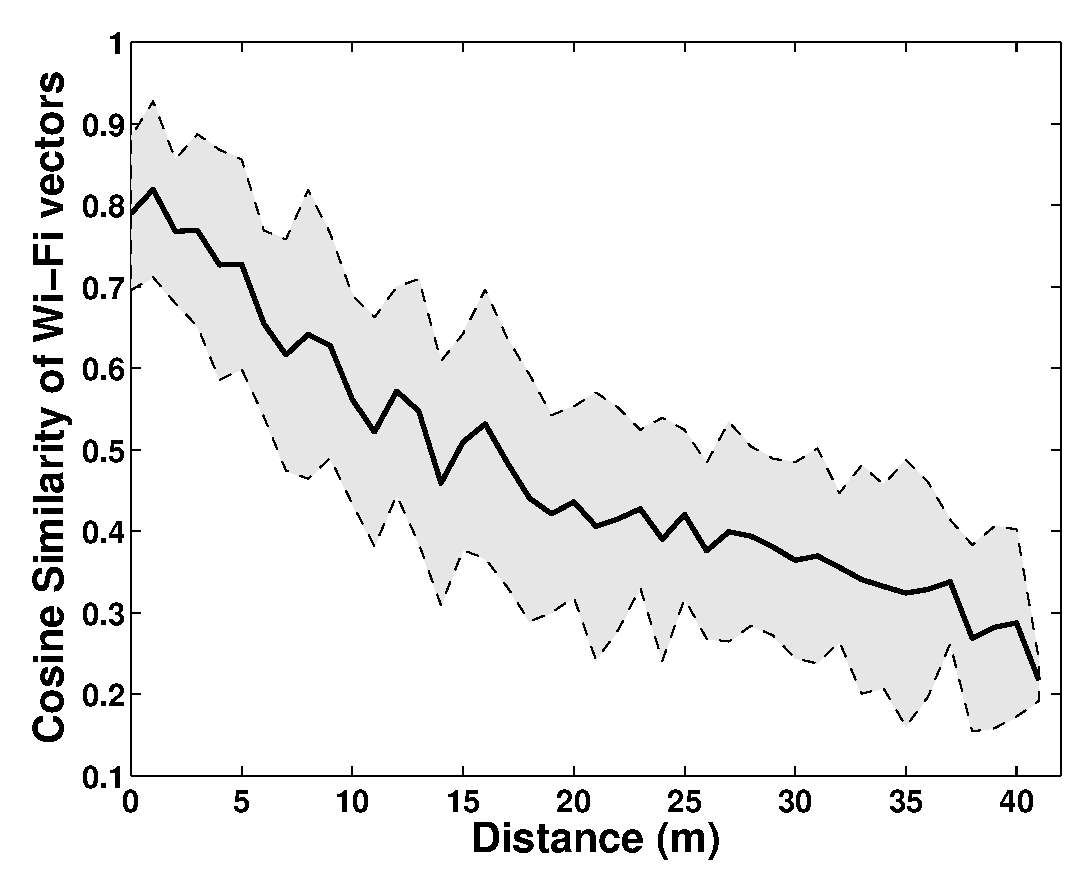
\includegraphics[width=.3\textwidth]{Figure1.eps}
\caption{Aggregate behavior of Wi-Fi Cosine Similarity against spatial distance as measured from various APs in B Hall. Results from other buildings were comparable and showed a similar trend}
\label{fig:wifi-similarity}
%\vspace{-17pt}
\end{figure}
%\vspace{-10pt}
To understand whether the similarity values are different at different locations, we collected Wi-Fi signatures at different points on a trajectory that starts to move away and return to the originating point. Specifically, we use Cosine Similarity between vectors as a measure of Wi-Fi similarity. 
Shown in Figure~\ref{fig:wifi-similarity} are aggregates of similarities in Wi-Fi vector space compared to the physical distance between locations from a building at our university. The trend clearly shows a coarse inverse correlation between physical distance and Wi-Fi similarity. This is expected since several models, including the ITU indoor propagation model, use this relation to find distance from RSSI values. 
%Similar observations regarding the spatial uniqueness of Wi-Fi signatures have been made by previous studies~\cite{biswas-icra10,thrun:cam-wifi} that perform indoor localization and we find them consistent with our analysis. %For example, \cite{yang-mobicom12} uses WiFi signatures to localize phones and \cite{biswas-icra10} uses them for both localization and navigation of mobile robots.
%\vspace{-5pt}
\subsection{Wi-Fi data processing}
{\bf Wi-Fi BSSID Dynamics: }An observation in RSSI aggregation is that each unique Access Point(AP) advertises different BSSIDs for different frequencies, 2.4GHz and 5GHz, and different access control mechanisms. These BSSIDs are only different in the last nibble of their MAC addresses. We aggregate all measurements from an AP by averaging the signal strength measured for all BSSIDs from a single AP.\\
{\bf Wi-Fi Data Collection:} The nature of Wi-Fi cards requires us to be stationary at a given location to collect steady signal strength readings. Therefore, during our measurements, our robot pauses for about ten seconds every few meters to collect Wi-Fi signals. \\
{\bf Wi-Fi Similarity Metric:}  The similarity between two different RSSI vectors $v$ and $w$ equals
%\begin{equation*}
$Similarity=\frac{v\cdot w}{\lvert v \rvert\lvert w \rvert}$. We use the cosine similarity measure in this work because it is invariant to scale. It is less sensitive to RSSI fluctuations due to configuration changes. \zaki{If some APs are unavailable at some respective position, we set the corresponding values to zero.}
%\end{equation*} 
